\documentclass[man]{apa6}

\usepackage{amssymb,amsmath}
\usepackage{ifxetex,ifluatex}
\usepackage{fixltx2e} % provides \textsubscript
\ifnum 0\ifxetex 1\fi\ifluatex 1\fi=0 % if pdftex
  \usepackage[T1]{fontenc}
  \usepackage[utf8]{inputenc}
\else % if luatex or xelatex
  \ifxetex
    \usepackage{mathspec}
    \usepackage{xltxtra,xunicode}
  \else
    \usepackage{fontspec}
  \fi
  \defaultfontfeatures{Mapping=tex-text,Scale=MatchLowercase}
  \newcommand{\euro}{€}
\fi
% use upquote if available, for straight quotes in verbatim environments
\IfFileExists{upquote.sty}{\usepackage{upquote}}{}
% use microtype if available
\IfFileExists{microtype.sty}{\usepackage{microtype}}{}

% Table formatting
\usepackage{longtable, booktabs}
\usepackage{lscape}
% \usepackage[counterclockwise]{rotating}   % Landscape page setup for large tables
\usepackage{multirow}		% Table styling
\usepackage{tabularx}		% Control Column width
\usepackage[flushleft]{threeparttable}	% Allows for three part tables with a specified notes section
\usepackage{threeparttablex}            % Lets threeparttable work with longtable

% Create new environments so endfloat can handle them
% \newenvironment{ltable}
%   {\begin{landscape}\begin{center}\begin{threeparttable}}
%   {\end{threeparttable}\end{center}\end{landscape}}

\newenvironment{lltable}
  {\begin{landscape}\begin{center}\begin{ThreePartTable}}
  {\end{ThreePartTable}\end{center}\end{landscape}}

  \usepackage{ifthen} % Only add declarations when endfloat package is loaded
  \ifthenelse{\equal{\string man}{\string man}}{%
   \DeclareDelayedFloatFlavor{ThreePartTable}{table} % Make endfloat play with longtable
   % \DeclareDelayedFloatFlavor{ltable}{table} % Make endfloat play with lscape
   \DeclareDelayedFloatFlavor{lltable}{table} % Make endfloat play with lscape & longtable
  }{}%



% The following enables adjusting longtable caption width to table width
% Solution found at http://golatex.de/longtable-mit-caption-so-breit-wie-die-tabelle-t15767.html
\makeatletter
\newcommand\LastLTentrywidth{1em}
\newlength\longtablewidth
\setlength{\longtablewidth}{1in}
\newcommand\getlongtablewidth{%
 \begingroup
  \ifcsname LT@\roman{LT@tables}\endcsname
  \global\longtablewidth=0pt
  \renewcommand\LT@entry[2]{\global\advance\longtablewidth by ##2\relax\gdef\LastLTentrywidth{##2}}%
  \@nameuse{LT@\roman{LT@tables}}%
  \fi
\endgroup}


  \usepackage{graphicx}
  \makeatletter
  \def\maxwidth{\ifdim\Gin@nat@width>\linewidth\linewidth\else\Gin@nat@width\fi}
  \def\maxheight{\ifdim\Gin@nat@height>\textheight\textheight\else\Gin@nat@height\fi}
  \makeatother
  % Scale images if necessary, so that they will not overflow the page
  % margins by default, and it is still possible to overwrite the defaults
  % using explicit options in \includegraphics[width, height, ...]{}
  \setkeys{Gin}{width=\maxwidth,height=\maxheight,keepaspectratio}
\ifxetex
  \usepackage[setpagesize=false, % page size defined by xetex
              unicode=false, % unicode breaks when used with xetex
              xetex]{hyperref}
\else
  \usepackage[unicode=true]{hyperref}
\fi
\hypersetup{breaklinks=true,
            pdfauthor={},
            pdftitle={Child language experience in a Tseltal Mayan village},
            colorlinks=true,
            citecolor=blue,
            urlcolor=blue,
            linkcolor=black,
            pdfborder={0 0 0}}
\urlstyle{same}  % don't use monospace font for urls

\setlength{\parindent}{0pt}
%\setlength{\parskip}{0pt plus 0pt minus 0pt}

\setlength{\emergencystretch}{3em}  % prevent overfull lines


% Manuscript styling
\captionsetup{font=singlespacing,justification=justified}
\usepackage{csquotes}
\usepackage{upgreek}

 % Line numbering
  \usepackage{lineno}
  \linenumbers


\usepackage{tikz} % Variable definition to generate author note

% fix for \tightlist problem in pandoc 1.14
\providecommand{\tightlist}{%
  \setlength{\itemsep}{0pt}\setlength{\parskip}{0pt}}

% Essential manuscript parts
  \title{Child language experience in a Tseltal Mayan village}

  \shorttitle{Child language experience in a Tseltal Mayan village}


  \author{Marisa Casillas\textsuperscript{1}, Penelope Brown\textsuperscript{1}, \& Stephen C. Levinson\textsuperscript{1}}

  % \def\affdep{{"", "", ""}}%
  % \def\affcity{{"", "", ""}}%

  \affiliation{
    \vspace{0.5cm}
          \textsuperscript{1} Max Planck Institute for Psycholinguistics  }

  \authornote{
    Correspondence concerning this article should be addressed to Marisa
    Casillas, Wundtlaan 1, 6525 XD Nijmegen, The Netherlands. E-mail:
    \href{mailto:Marisa.Casillas@mpi.nl}{\nolinkurl{Marisa.Casillas@mpi.nl}}
  }


  \abstract{Enter abstract here. Each new line herein must be indented, like this
line.}
  \keywords{keywords \\

    \indent Word count: X
  }





\usepackage{amsthm}
\newtheorem{theorem}{Theorem}[section]
\newtheorem{lemma}{Lemma}[section]
\theoremstyle{definition}
\newtheorem{definition}{Definition}[section]
\newtheorem{corollary}{Corollary}[section]
\newtheorem{proposition}{Proposition}[section]
\theoremstyle{definition}
\newtheorem{example}{Example}[section]
\theoremstyle{definition}
\newtheorem{exercise}{Exercise}[section]
\theoremstyle{remark}
\newtheorem*{remark}{Remark}
\newtheorem*{solution}{Solution}
\begin{document}

\maketitle

\setcounter{secnumdepth}{0}



\section{Introduction}\label{introduction}

\begin{itemize}
\tightlist
\item
  Children require linguistic input to become full-fledged speakers of
  their language(s)
\item
  As developmentalists, our ultimate goal is to be able to model the
  diverse mechanisms that allow children to convert the linguistic
  information in their environment to internalized linguistic knowledge,
  e.g., (statistical learning, motor development, etc.; see slides)
\item
  We have (rightfully) spent an enormous amount of time analyzing what
  information exists in children's input---such information is an
  important jumping off point for inspiring and constraining theories
  about learning mechanisms
\item
  We have developed many techniques for tracking input, most recently
  daylong recordings
\item
  Extoll the virtues of daylong recordings
\item
  Indeed, studies along these lines, linking children's language
  experience to their language outcomes, finds a strong impact of
  experience, especiall with respect to CDS

  \begin{itemize}
  \tightlist
  \item
    List some findings on input effects
  \item
    Why is CDS special? Briefly list findings
  \end{itemize}
\item
  However, there are two major caveats to this work, all interrelated
  with each other:
\item
  1: While evidence linking input and vocab is super strong, evidence
  linking input to grammar is more scant; aspects of the system may be
  differentially sensitive to experience (Dan's paper)
\item
  2: Literacy-centric view of language development; what is the
  \enquote{target}?
\item
  3: Focused on WEIRD kids
\item
  A key avenue for addressing these issues is to promote further study
  of lg development in non-WEIRD contexts.
\item
  Linguistic anthropologists have been doing this for a long time
\item
  Now it's time for us to follow-up using our own methods so that we can
  more feasibly compare

  \begin{itemize}
  \tightlist
  \item
    Though that comes with its own problems (cite\ldots{})
  \end{itemize}
\item
  Especially in less-literate/semi-literate communities, it lets us more
  easily think about language acquisition apart from literacy
\item
  In this paper we examine the linguistic experiences of 10 Tseltal
  Mayan children. Why Mayan?
\item
  Non-WEIRD
\item
  Rich area of research: Little CDS from report---potentially a great
  case for looking at a functioning acquisition system with minimal
  environmental input
\item
  Many linguistically and culturally similar communities for comparison
  (see Shneidman, Pye, etc.)
\item
  See slides for more
\item
  A major contribution of this work is to use daylong recordings, which
  allow us to estimate\ldots{} (TLM paper on short vs.~longer recs).

  \begin{itemize}
  \tightlist
  \item
    At the same time, there is potentially great value in knowing about
    what happens during interactional bursts when they happen, so we
    track \ldots{} tt and va as well
  \end{itemize}
\item
  Our aim is to develop a child language environment profile for Tseltal
  Mayan, one that gives an impression of the speech children hear around
  them and the type of speech that is addressed to them directly. 
\item
  Results:
\item
  How much speech do children hear overall and what proportion of that
  is directed to them? How does that compare to other communities we've
  studied?

  \begin{itemize}
  \tightlist
  \item
    \emph{measures}: XDS and TDS minutes per hour and proportion (from
    random selections only)
  \end{itemize}
\item
  How do ADS and TDS differ?

  \begin{itemize}
  \tightlist
  \item
    \emph{measures}: utt length, repetitiveness, F0 peaks and ranges,
    questions, imperatives (?)
  \end{itemize}
\item
  How much speech do children hear during bouts/bursts of interaction?
  How often do these bursts occur?

  \begin{itemize}
  \tightlist
  \item
    \emph{measures}: deltas for m/h TDS, \#utts TDS, \# TT transitions
    between random, tt, and va: are they actually different?
  \item
    \emph{measures}: XDS and TDS minutes per hour and proportion (from
    tt and va selections: do they show similar age effects?)
  \item
    \emph{measures}: sliding window in random to match mean TDS rate/TT
    transition rates
  \end{itemize}
\item
  Does interaction influence linguistic practice?

  \begin{itemize}
  \tightlist
  \item
    \emph{measures}: m/h CHI vocs, \# CHI vocs, \& voc mat between
    random, tt, and va
  \end{itemize}
\item
  Discussion
\item
  Summary of findings
\item
  When thinking about quantity: Do we care about the avg over the day or
  do bursts matter more?

  \begin{itemize}
  \tightlist
  \item
    Benefits of naps between bursts? Natural input cycle? How many
    \enquote{good} minutes are enough to spur learning on?
  \end{itemize}
\item
  How should we think about CDS? What is universal about its format?
\item
  So what is the impact of input in this community? What do we predict?

  \begin{itemize}
  \tightlist
  \item
    One point often raised: do these kids show a delay? Problematize
    this.
  \item
    More interesting: language experience itself shapes use of
    mechanisms for learning, e.g., learning fro overhearing (Shneidman)
  \end{itemize}
\item
  Big issue we have to face as work continues in this vein: what are
  these kids learning? We can't continue to pretend that we are capable
  of defining and encapsulating a phenomenon as emergent as language.
\item
  Limitations

  \begin{itemize}
  \tightlist
  \item
    no video data
  \item
    only 10 kids
  \end{itemize}
\end{itemize}

\section{Methods}\label{methods}

\subsection{Participants}\label{participants}

\subsection{Material}\label{material}

\subsection{Procedure}\label{procedure}

\subsection{Data analysis}\label{data-analysis}

\section{Results}\label{results}

\begin{figure}
\centering
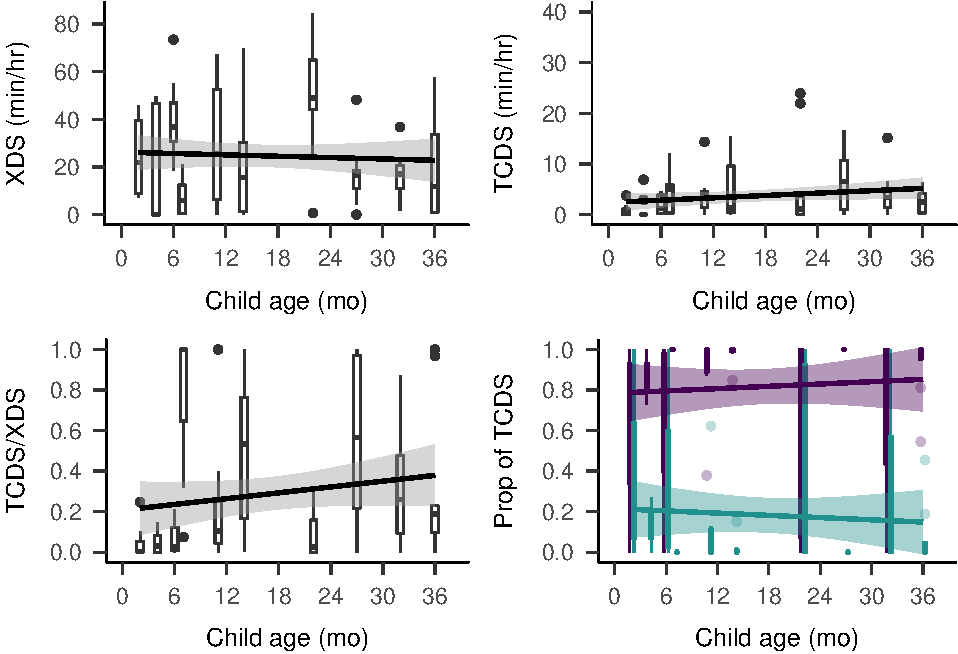
\includegraphics{Tseltal-CLE_files/figure-latex/plot_XDS_TDS_quantity_random-1.pdf}
\caption{}
\end{figure}

\begin{figure}
\centering
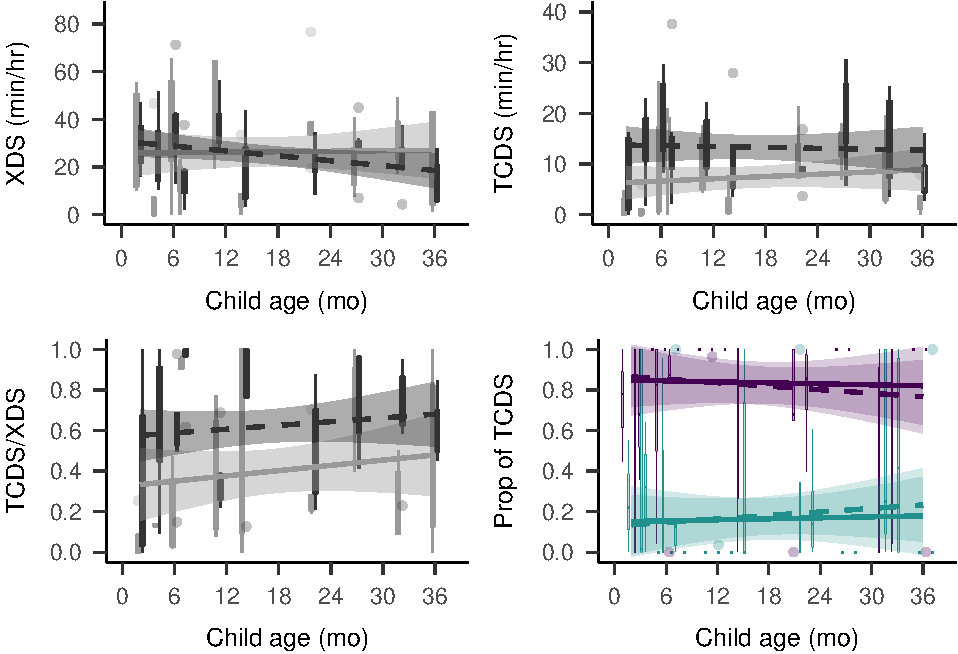
\includegraphics{Tseltal-CLE_files/figure-latex/plot_XDS_TDS_quantity_nonrandom-1.pdf}
\caption{}
\end{figure}

\section{Discussion}\label{discussion}

\newpage

\section{References}\label{references}

\begingroup
\setlength{\parindent}{-0.5in} \setlength{\leftskip}{0.5in}

\hypertarget{refs}{}

\endgroup






\end{document}
